\newpage

\part{Testing}  

    \graphicspath{{images/testing/}}

    Further evidence for the tests can be found in the appendix. A google drive folder where video evidence of the tests can be found here: \url{https://bit.ly/2WyO9L0}.

    All time-based tests were done by changing the system time, as is shown in the videos. Please note that the time changed was in GMT whereas the server was getting the UTC time. At points these don’t match up when the test time passed between GMT and BST.

    Any tests that included modifying the database or any stored files show the data in each file before and after the test.


    \section{Predictions}
        Testing the networks was difficult as there was no solid idea of how a well-trained network "should" act on given data as the forex market is stochastic. We can however evaluate the performance of each network on historic data as well as try to evaluate the networks' abilities to determine and follow trends using fabricated data.

        \subsection{Performance on Unseen Data}
        The following repeats the results shown in the final design section. \textit{See A.1} for sample graphs of the test data against predictions made.

        \begin{tabular}{|p{2cm}|p{1.5cm}|p{1.5cm}|p{2.5cm}|p{2.5cm}|}
            \hline
            Timestep & Window Size & Layer number & Percentage Performance & Mean Squared Error\\
            \hline
            \multirow{15 (15*1)}
            & - & - & - & 0.0047292\\
            & 5 & 20 & 92.586 & 0.0047001\\
            \hline
            \multirow{30 (15*2)}
            & - & - & - & 0.0091900\\
            & 10 & 20 & 91.979 & 0.0091604\\
            \hline
            \multirow{60 (15*4)}
            & - & - & - & 0.018476 \\
            & 20 & 30 & 87.311 & 0.018470 \\
            \hline
            \multirow{120 (15*8)}
            & - & - & - & 0.037538\\
            & 40 & 30 & 88.181 & 0.037942\\
            \hline
            \multirow{240 (15*16)}
            & - & - & - & 0.0047292 \\
            & 65 & 30 & 81.197 & 0.076780 \\
            \hline
            \multirow{480 (15*32)}
            & - & - & - & 0.14996 \\
            & 90 & 30 & 69.199 & 0.15115\\
            \hline
        \end{tabular}

        \subsection{Analysis of Behaviour on Simple Trends}
        The following tests examine how all the networks viewed together perform on simple trends. It was thought this would help give a better (qualitative) understanding of how the networks performed. 3 scenarios were used - straight line positive gradient, straight of line negative gradient (to test if behaviour is roughly symmetrical for upwards/downwards movements) and a sine wave. 

        In addition, tests were done where "noise" was included by randomly adding from -5 to 5 pips to the value that the trend should be. For all tests, the open/close price were values given by the function producing the trend and the high/low price were calculated by adding/subtracting 0.005 to the close price of a timestep.

            \subsubsection{Straight Line}
            Graphs of the networks' predictions on straight lines without noise were as follows. The close prices of the data fed to the networks is shown in blue and predictions are shown as lines connected between every price point and shown in orange.

            \begin{figure}[htbp]
                \centering
                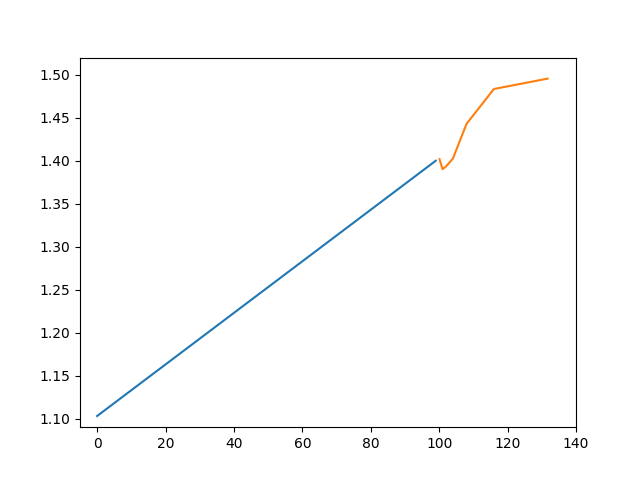
\includegraphics[width=0.9\textwidth]{asc.png}
                \caption{Predictions on a straight line (positive gradient)}
                \label{fig:asc}
            \end{figure}

            From the above, we can see that the networks on the whole were very good at predicting the upwards trends. Surprisingly however, it appears as though the prediction for 32 timesteps or 8 hours in the future (the final prediction) was actually the best at matching the trends but the predictions made for 1, 2 and 4 timesteps or 15, 30 and 60 minutes respectively were worst at this. It was thought that this is because the window size that these networks used were far smaller than the others. As the market is so volatile, If there is a steady price increase in the short term, it is quite likely that the price will in fact drop. This is potentially as a large number of traders on seeing this increase will start to short the asset to try to capitalise on this or due to traders setting buy orders on upper bounds of the price. 

            Additionally, it is very reassuring to see that behaviour does indeed appear to be symmetrical for price increases and decreases. 

            \begin{figure}[htbp]
                \centering
                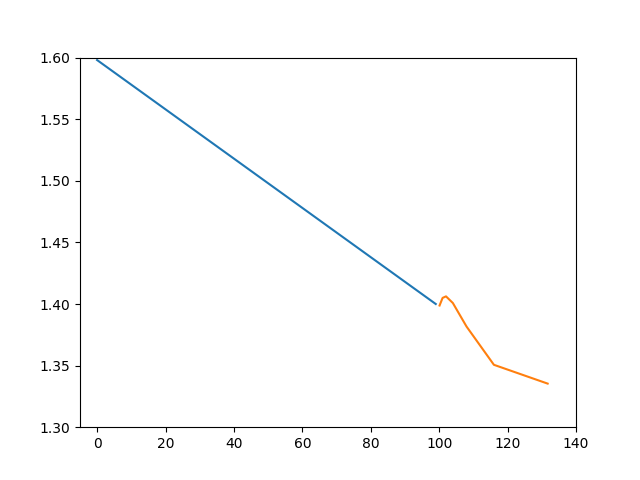
\includegraphics[width=0.9\textwidth]{dsc.png}
                \caption{Predictions on a straight line (negative gradient)}
                \label{fig:dsc}
            \end{figure}

            Also very reassuringly, adding noise appears to have very little impact on the predictions, with the only visible differences seen in the shorter term predictions which is to be expected given the smaller windows they use. 

            \begin{figure}[htbp]
                \centering
                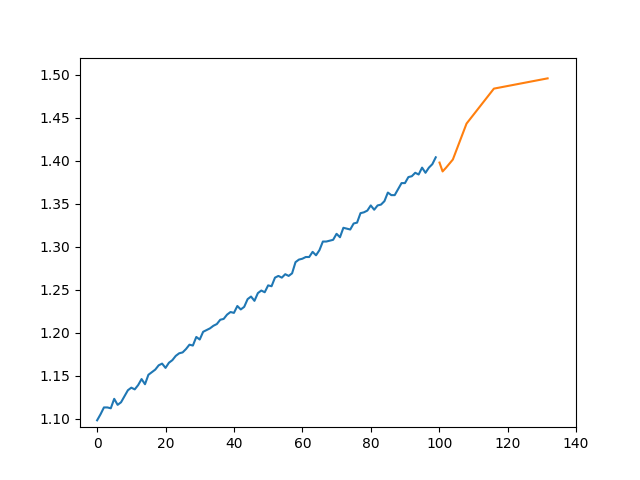
\includegraphics[width=0.9\textwidth]{ascNoise.png}
                \caption{Predictions on a straight line with noise (positive gradient)}
                \label{fig:ascNoise}
            \end{figure}

            \begin{figure}[htbp]
                \centering
                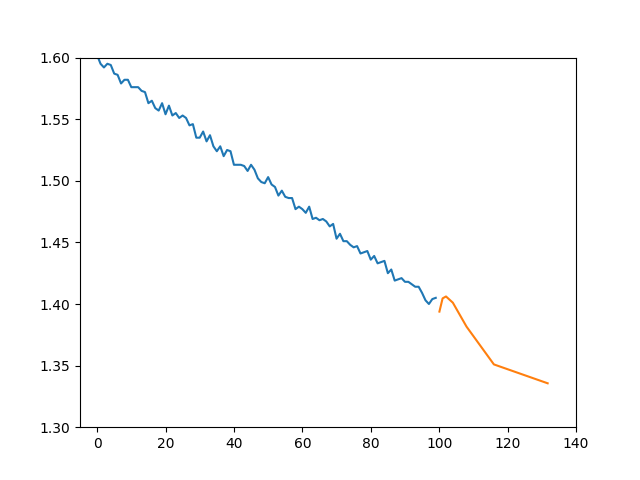
\includegraphics[width=0.9\textwidth]{dscNoise.png}
                \caption{Predictions on a straight line with noise (negative gradient)}
                \label{fig:dscNoise}
            \end{figure}

            \newpage
            \subsubsection{Sine Wave}
            For the tests on the sine waves, it was felt the most useful, and potentially most difficult test would be trying to predict future prices given data just before a peak or trough. This is to see if the networks were able to pick up on the steadily increasing or decreasing gradients and make predictions accordingly. Given the tests above showed that the behaviour was symmetrical for price increases/decreases, only one set of tests is shown below.

            \begin{figure}[htbp]
                \centering
                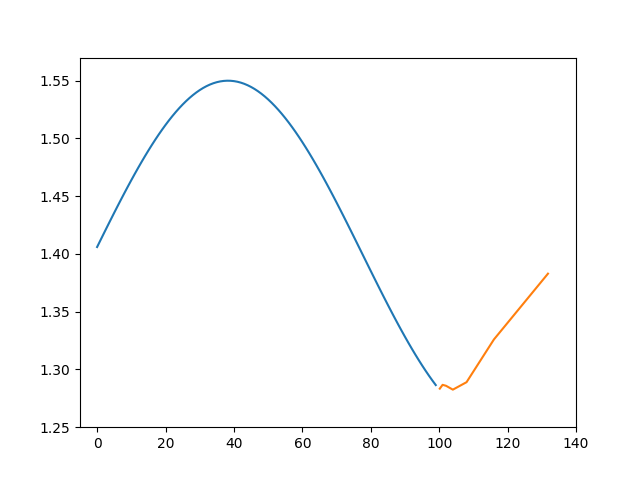
\includegraphics[width=0.9\textwidth]{sine.png}
                \caption{Predictions on a sine wave}
                \label{fig:sine}
            \end{figure}

            \begin{figure}[htbp]
                \centering
                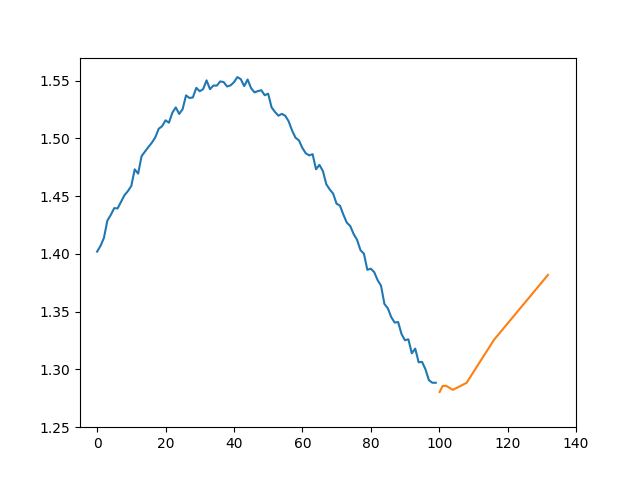
\includegraphics[width=0.9\textwidth]{sineNoise.png}
                \caption{Predictions on a sine wave with noise}
                \label{fig:sineNoise}
            \end{figure}

            Again we see that the shorter term networks have sometimes predicted movements in opposition to what would be expected, likely for the same reasons as above. The longer term prediction exceeded any expectations of how they would perform, determining the upwards trend surprisingly well. Again, it is shown that noise makes little impact to the networks' abilities to pick up on the trends in the longer term.

            \subsubsection{Comments on the tests}
            These tests show that the networks on the whole, were very good at predicting trends. It was shown that they were in fact giving "useful" predictions instead of just quoting the most recent close price. Initially it was surprising to see that the longer term predictions appeared to perform better than shorter term ones on the upwards and downwards trends however this was thought to be justified given the shorter windows used by the shorter term predictions as well as the nature of the market.

        \subsection{Parsing data to networks}
        The dimensions of data returned were calculated in the following way. For the n availiable datapoints the number of paris of inputs/targets m is given by:
        
        \begin{equation}
        m = n - timestepToPredict - windowSize + 1
        \end{equation}

        Thus when splitting, there should be splitProp * m sets of training inputs/tagets.
        The number of inputs considered for a given m number of input/target pairs is given by:

        \begin{equation}
            inputNo = m + windowSize - 1
        \end{equation}

        For each m set of inputs/targets there is one mean calculated that is used to normalise the inputs i.e number of means = m

        The following tests check that data is being correctly formatted to be input to the networks.

        \begin{tabular}{|p{1cm}|p{4cm}|p{4cm}|p{2cm}|}
            \hline
            testID & Input & Expected Output & Passed\\
            \hline
            1.1 & call process.get(3, 2, "twentyLines.csv"), (windowSize of 3, timestepToPredict 2) splitProp of 0.8 & Returned dimensions: 14/6 training/testing inputs, 12/4 training/testing means, 12/4 training/testing targets&Y\\
            \hline 
            1.2 & call process.get(3, 2, "twentyLines.csv"), splitProp of 0.8 & Returned values: training inputs are first 14 datapoints, test inputs' first windowSize-1 inputs are last windowSize-1 training inputs, ith target is the (windowSize+timestepToPredict)th close price&Y\\
            \hline 
            1.3 & call getBatch on the test inputs, means, targets (batchProp 0.5) & Returned dimensions: 2 sets of windows (inputs), 2 targets&Y\\
            \hline 
            1.4 & call getBatch on the test inputs, means, targets (batchProp 0.5) & Returned values: All values betweem -1 and 1 &Y\\
            \hline 
        \end{tabular} 


        \section{Site}
        \subsection{Navigation}
        \begin{tabular}{|p{1cm}|p{4cm}|p{4cm}|p{2cm}|}
            \hline
            testID & Test & Expected Outcome & Passed\\
            \hline
            2.1.1 & Load site & Home page shown & Y\\
            \hline 
            2.1.2 & Click on "About" & About page shown & Y\\ 
            \hline 
            2.1.3 & Click on "API" & API page shown & Y\\ 
            \hline 
            
        \end{tabular} 

        \subsection{Main Page}
        \begin{tabular}{|p{1cm}|p{4cm}|p{4cm}|p{2cm}|}
            \hline
            testID & Test & Expected Outcome & Passed\\
            \hline
            2.2.1 & Load page & "Current time" shows the current time, "Showing data for" corresponds to the current data being shown. Current data being shown matches the most recent availiable data & Y\\
            \hline
            2.2.2 & Move prediction range slider & Text-box value updates and chart redraws with corresponding number of predictions & Y\\
            \hline 
            2.2.3 & Move historic range slider & Text-box value updates and chart redraws with corresponding number of historic data points & Y\\
            \hline 
            2.2.4 & Load site after 10pm on Friday & Weekend message shown & Y\\
            \hline
            2.2.5 & Load site after 10pm on Sunday & Weekend message not shown & Y\\
            \hline
        \end{tabular} 
    
        \subsection{API signup}
        \begin{tabular}{|p{1cm}|p{4cm}|p{4cm}|p{2cm}|}
            \hline
            testID & Test & Expected Outcome & Passed\\
            \hline
            2.3.1 & Enter "hello" into email field & Javascript alert seen & Y\\
            \hline 
            2.3.2 & Enter "test@gmail.com" & Redirected to API key page and key is shown & Y\\ 
            \hline
            2.3.3 & Enter "test@gmail.com" again & Page is reloaded with message and API key shown & Y\\
            \hline
            2.3.4 & Click "example query" & sample.json shown & Y\\
            \hline
            2.3.5 & Check database & new user with apikey retrieved earlier shown & Y\\
            \hline
        \end{tabular} 

    \section{API}
    \begin{tabular}{|p{1cm}|p{4cm}|p{4cm}|p{2cm}|}
        \hline
        testID & Test & Expected Outcome & Passed\\
        \hline
        3.1 & Use key tied to "test@gmail.com" & Current predictions.json file returned & Y\\
        \hline 
        3.2 & Immediately request with the same API key again & invalidGet.json returned & Y\\ 
        \hline
        3.3 & Request with invalid API key & invalidGet.json returned & Y\\
        \hline
        3.4 & Request with no API key & invalidGet.json returned & Y\\
        \hline
        3.5 & Check database & 2 requests from user\_id 1, one of them one served, one not. Requests with invalid keys not shown in database& Y\\
        \hline
        3.6 & Make request with API key tied to "test@gmail.com" again (more than 20 seconds after previous) & Request served and request saved in database &Y\\
        \hline
    \end{tabular} 

    \section{Updates}
    The last 4 tests below test the purging of inactive users stats retrieved at midnight. These tests follow from those carried out in the API section (keeping the user with API key associated to "test@gmail.com" along with the requests made by them). For the first three of these a user is first added over a month before the current date. They should make two requests within 20 seconds of each other. This is to test that the purging of inactive users works as expected and that stats retrieved are only from the last day. For the last test, a new user is also added however it is expected that the user should not be removed. 

    \begin{tabular}{|p{1cm}|p{4cm}|p{4cm}|p{2cm}|}
        \hline
        testID & Test & Expected Outcome & Passed\\
        \hline\hline
        & \textbf{Normal Operation} & &\\
        \hline
        4.1.1 & Current time is a "multiple" of 15 minutes & Server tries to update the price data & Y\\
        \hline 
        4.1.2 & Timestamp of data received is the same as the data currently stored & Old data is kept, keep checking for updated data & Y\\
        \hline
        4.1.3 & When new data is received & New data is saved to the file & Y\\
        \hline
        4.1.4 & When new data is received & Predictions are made and updated in less than 30 seconds & Y\\
        \hline
        4.1.5 & Check database & New prediction entry has been added & Y\\
        \hline
        4.1.6 & Run flask app & Server checks for new prices immediately when first request is made & Y\\
        \hline\hline
        & \textbf{Erroneous Price Data} & &\\
        \hline
        4.2.1 & Data received has key "Error" & Old data is kept, keep checking for updated data & Y\\
        \hline
        4.2.2 & Data received has key "Note"& Old data is kept, keep checking for updated data & Y\\
        \hline
        4.2.3 & Data received is in .csv format & Old data is kept, keep checking for updated data & Y\\
        \hline
        4.2.4 & Bad connection and so no data retrieved & Old data is kept, keep checking for updated data & Y\\
        \hline\hline
        & \textbf{Midnight updates} & &\\
        \hline
        4.3.1 & At midnight & atMidnight function called & Y\\
        \hline
        4.3.2 & At midnight & Console displays: 1 new user signed up, 1 user removed, 1 remaining user, 1 active user, 3 total requests, 1 rejected request & Y \\
        \hline
        4.3.3 & Check database & Inactive user removed & Y\\
        \hline
        4.3.4 & Call Purge when a user has been inactive for 29 days & User not removed & Y\\
        \hline
    \end{tabular}